\section{The Game}
\label{sec:game}

\subsection{Concept and structure}

The artefact is a web-based, single-session educational game that supports the understanding of Nielsen's ten heuristics through paired interactive scenarios. For each heuristic, the player completes the same concrete task in two interfaces: one that violates the heuristic, and one that respects it. A narrator frames each interaction before and after, and a reveal screen at the end of the pair names the heuristic and explains it through the contrast between the two interfaces. The game is bilingual (English and Portuguese) and runs entirely in the browser, with no server-side state.

Each of the ten heuristics follows the same five-step flow. The player first sees a \emph{goal card} stating the concrete task to be performed. They then enter the \emph{bad scenario}, where the narrator presents the goal and the task is carried out in an interface that violates the heuristic; after completing the task, the narrator returns to comment on what just happened. The same task is then repeated in the \emph{good scenario}, with the narrator framing the interaction before and after in an interface that respects the heuristic. A \emph{reveal screen} closes the pair, naming the heuristic, presenting its definition, and recapping the contrast side by side; the player is awarded a star and advances to the next heuristic. After all ten heuristics have been completed, a celebratory closing screen greets the player as a ``heuristics expert'' and a final results screen links to the post-game questionnaire described in Section~\ref{sec:method}.

To make this flow concrete, Figures~\ref{fig:h8-bad}, \ref{fig:h8-good}, and~\ref{fig:h8-reveal} show the full sequence for heuristic 8, \emph{Aesthetic and Minimalist Design}, whose task is to find and click the ``Buy Now'' button for a specific laptop on a shop page.

\begin{figure}[ht]
\centering
\pdftooltip{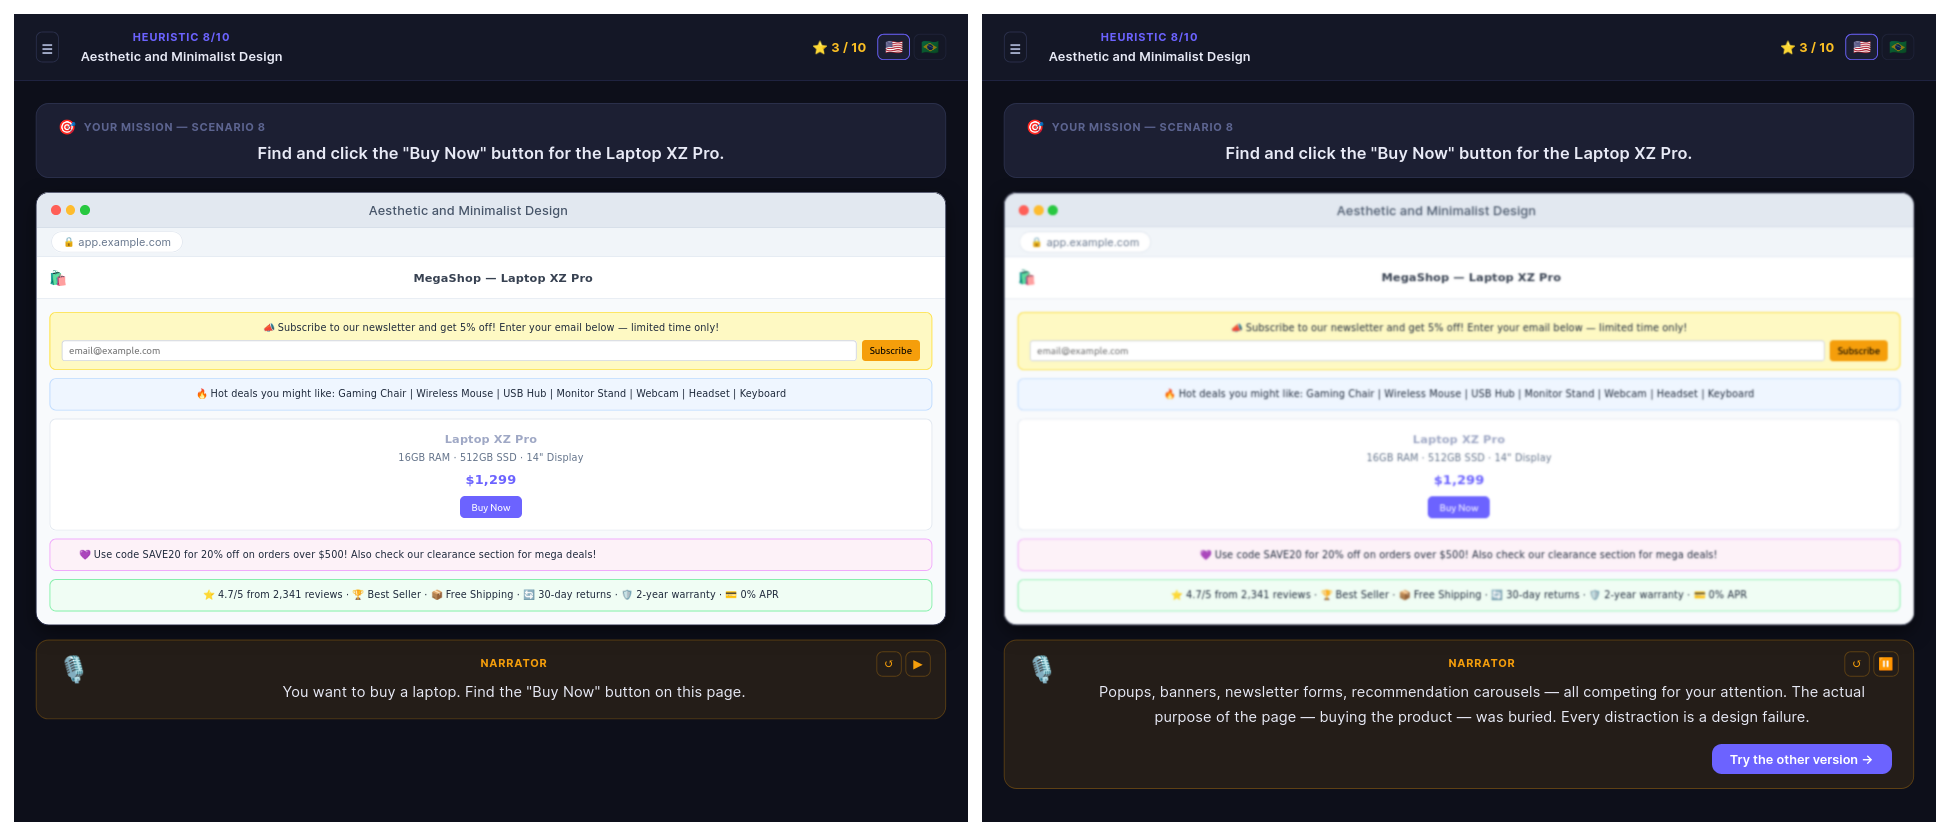
\includegraphics[width=.95\textwidth]{figures/h8-bad-scenario-after-and-before.png}}
{Two side-by-side screenshots of the bad scenario for heuristic 8 (Aesthetic and Minimalist Design). On the left, the player enters the scenario: the mission ``Find and click the Buy Now button for the Laptop XZ Pro'' appears at the top, above a cluttered shop interface with overlapping yellow newsletter banners, recommendation carousels of unrelated products, deal labels, and prices that obscure the actual product. The narrator at the bottom says: ``You want to buy a laptop. Find the Buy Now button on this page.'' On the right, the same interface is shown after the task is completed; the narrator now comments: ``Popups, banners, newsletter forms, recommendation carousels --- all competing for your attention. The actual purpose of the page --- buying the product --- was buried. Every distraction is a design failure.''}
\caption{Bad scenario for heuristic 8 (Aesthetic and Minimalist Design): the player's mission and the cluttered interface they meet (left), and the narrator's commentary after the task is completed (right).}
\label{fig:h8-bad}
\end{figure}

\begin{figure}[ht]
\centering
\pdftooltip{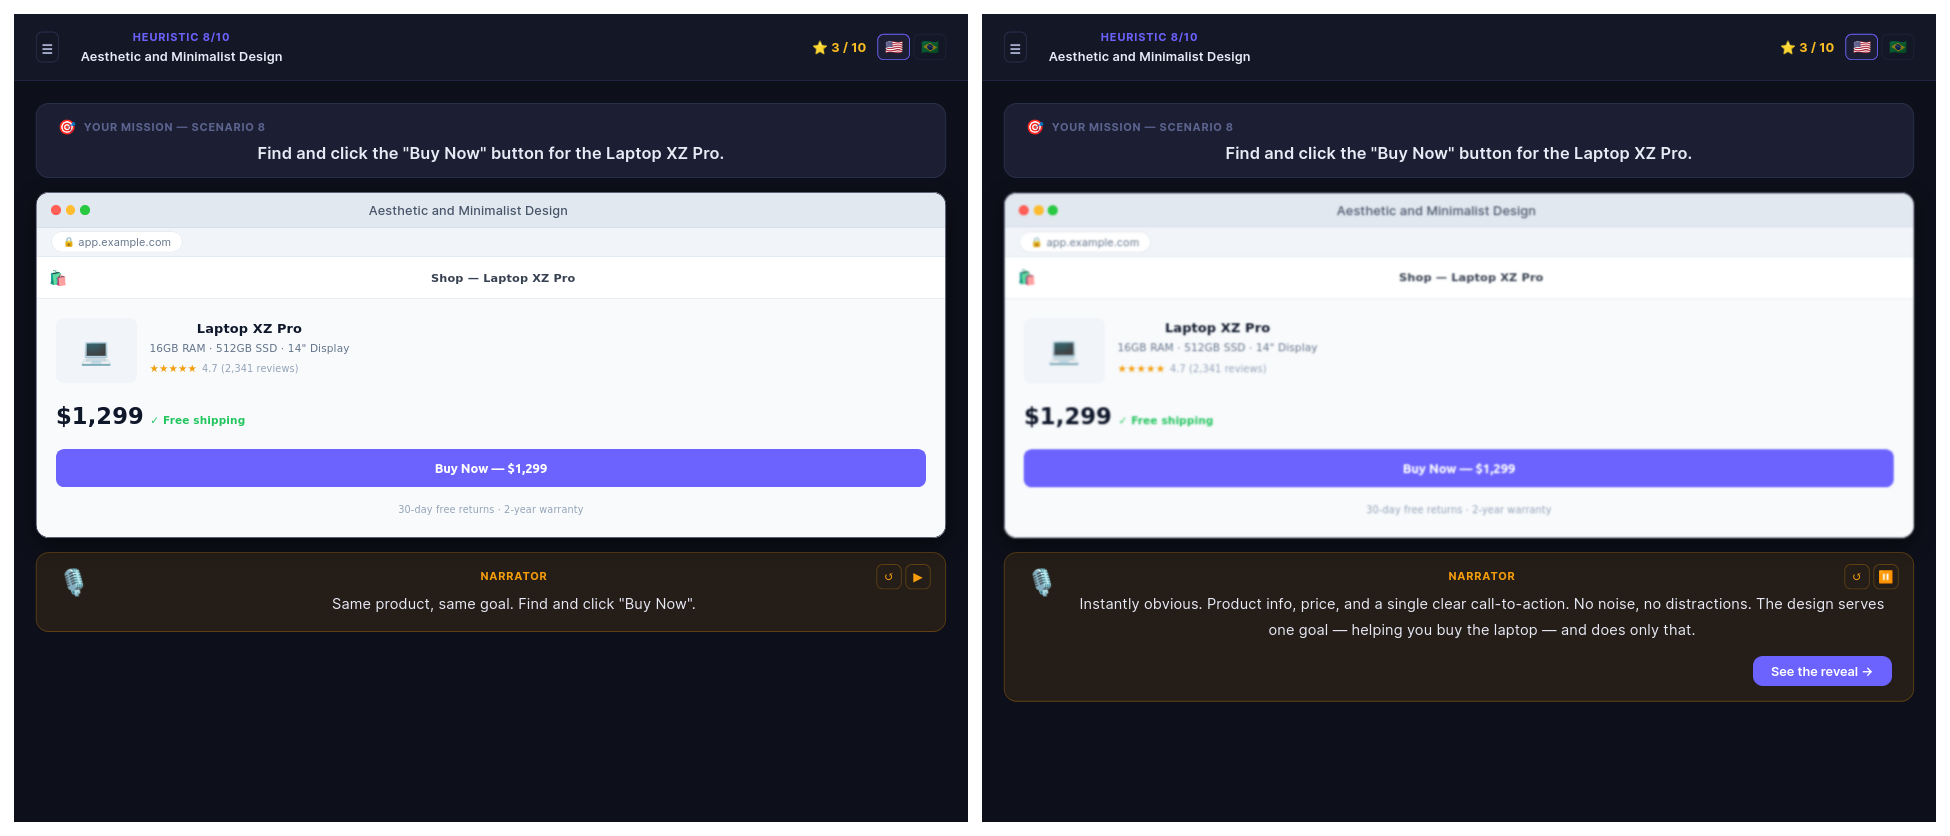
\includegraphics[width=.95\textwidth]{figures/h8-good-scenario-after-and-before.png}}
{Two side-by-side screenshots of the good scenario for heuristic 8 (Aesthetic and Minimalist Design). On the left, the player enters the scenario with the same mission ``Find and click the Buy Now button for the Laptop XZ Pro'' at the top, but the interface below is now minimal: a single product card for the Laptop XZ Pro showing its name, specifications (16 GB RAM, 512 GB SSD, 14-inch display), a 4.7-star rating, the price (\$1,299) with free shipping, and a single prominent purple ``Buy Now --- \$1,299'' button below. The narrator says: ``Same product, same goal. Find and click Buy Now.'' On the right, the same interface is shown after the task is completed; the narrator now comments: ``Instantly obvious. Product info, price, and a single clear call-to-action. No noise, no distractions. The design serves one goal --- helping you buy the laptop --- and does only that.''}
\caption{Good scenario for heuristic 8 (Aesthetic and Minimalist Design): the same mission in a minimal interface (left), and the narrator's commentary after the task is completed (right).}
\label{fig:h8-good}
\end{figure}

\begin{figure}[ht]
\centering
\pdftooltip{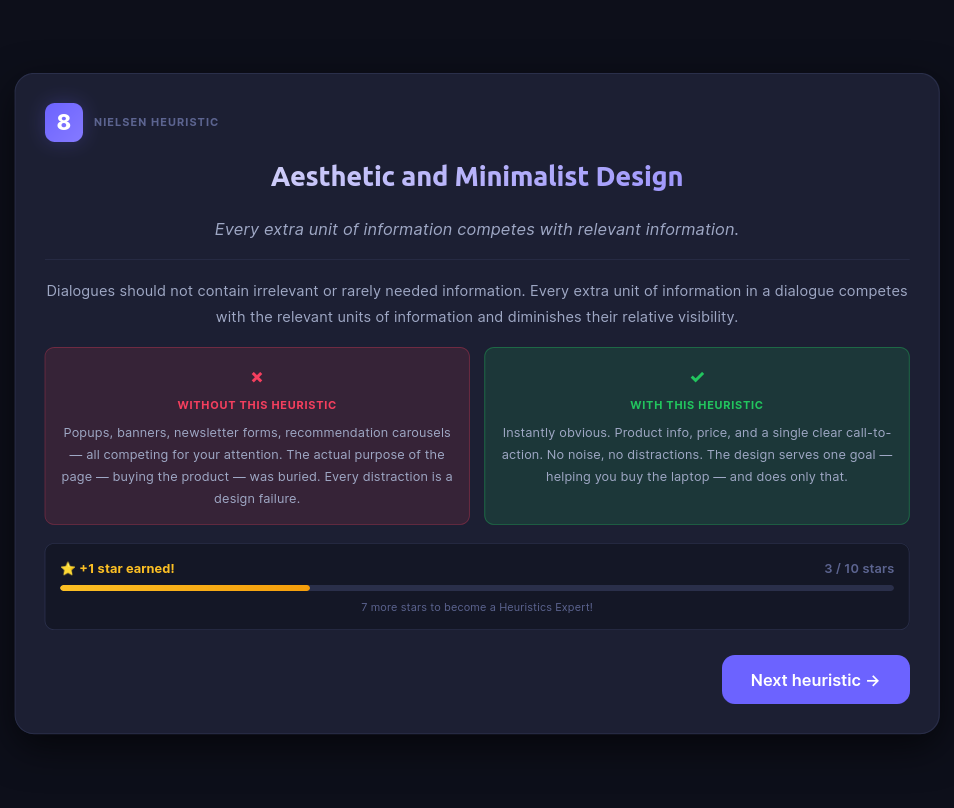
\includegraphics[width=.75\textwidth]{figures/h8-reveal-screen.png}}
{Reveal screen for heuristic 8 (Aesthetic and Minimalist Design). At the top, the heuristic number ``8'' and the label ``Nielsen Heuristic'' precede the heuristic title ``Aesthetic and Minimalist Design''. Below, the tagline reads ``Every extra unit of information competes with relevant information.'', followed by Nielsen's full definition: ``Dialogues should not contain irrelevant or rarely needed information. Every extra unit of information in a dialogue competes with the relevant units of information and diminishes their relative visibility.'' Two side-by-side coloured cards then recap the contrast: on the left, a red ``Without this heuristic'' card explains that popups, banners, newsletter forms, and recommendation carousels competed for the player's attention and buried the actual purpose of the page; on the right, a green ``With this heuristic'' card explains that product info, price, and a single clear call-to-action made the goal instantly obvious. At the bottom, a yellow progress bar indicates ``+1 star earned'' and shows the running total of 3 out of 10 stars, with the message ``7 more stars to become a Heuristics Expert!''. A purple ``Next heuristic'' button sits at the bottom right.}
\caption{Reveal screen for heuristic 8: the heuristic is named and defined, the contrast between the two scenarios is recapped, and a star is awarded.}
\label{fig:h8-reveal}
\end{figure}

\subsection{The ten heuristics}

The ten heuristics covered by the game follow the consolidated formulation by Nielsen~\cite{nielsen1994heuristic,nielsen2024tenheuristics}. Each heuristic is paired with a concrete, self-contained task that can be carried out by the player in a few clicks within a single screen. The bad and the good scenario for the same heuristic use the same task, but the interface around it is intentionally redesigned so that the contrast between violating and respecting the heuristic is directly visible in the interaction. Table~\ref{tab:heuristics} lists the heuristics in the order in which they appear in the game, the task used in each pair of scenarios, and the specific design contrast between the violating and the compliant interface.

{
\footnotesize
\setlength{\tabcolsep}{4pt}
\begin{longtable}[c]{c|p{2.3cm}|p{2.5cm}|p{4.0cm}|p{4.0cm}}
  \caption{The ten Nielsen heuristics, the concrete task used in each pair of scenarios, and the design contrast between the violating (bad) and the compliant (good) interface.}
  \label{tab:heuristics}\\
  \hline
  \textbf{\#} & \textbf{Heuristic} & \textbf{Task} & \textbf{Bad scenario} & \textbf{Good scenario} \\
  \hline
  \endfirsthead

  \multicolumn{5}{l}{\textit{Table~\thetable\ --- continued from previous page}}\\
  \hline
  \textbf{\#} & \textbf{Heuristic} & \textbf{Task} & \textbf{Bad scenario} & \textbf{Good scenario} \\
  \hline
  \endhead

  \hline
  \multicolumn{5}{r}{\textit{Continued on next page}}\\
  \endfoot

  \hline
  \endlastfoot

  1 & Visibility of System Status & Send a message to a friend about dinner tonight. & No feedback while the message is sending; the user cannot tell whether it went through. & A progress bar followed by a ``Message delivered'' confirmation keeps the user informed at every step. \\
  \hline
  2 & Match Between System and the Real World & Save the document before closing. & Buttons labelled ``Serialize \& commit to persistent storage layer'' and ``Discard volatile in-memory state'' force the user to decode technical jargon. & Plain-language labels such as ``Save'' and ``Discard changes'' use the vocabulary people actually think in. \\
  \hline
  3 & User Control and Freedom & Exit an accidentally opened upgrade wizard without completing the upgrade. & No cancel, close, or back option on the first step --- the user must either complete the upgrade or abandon the session. & Multiple clearly marked exits (a close button, a cancel link on every step, and a confirmation dialog) let the user leave at any point. \\
  \hline
  4 & Consistency and Standards & Navigate through all four checkout steps. & Navigation buttons change label (``Proceed'', ``Go on'', ``Continue'') and position from step to step, forcing the user to re-learn the interface at every screen. & Identical ``Back'' and ``Next'' buttons in the same position on every step. \\
  \hline
  5 & Error Prevention & Delete the account from settings. & A single click permanently deletes the account, with no warning or confirmation. & Several protective layers --- a de-emphasised button, a warning dialog, a type-to-confirm field, and an acknowledgement checkbox --- prevent accidental deletion. \\
  \hline
  6 & Recognition Rather Than Recall & Make the word ``important'' bold in a document. & Toolbar buttons are labelled only ``1'', ``2'', and ``3'', with no indication of what they do; the user has to memorise or guess. & Visible, familiar formatting controls let the user recognise the correct action immediately. \\
  \hline
  7 & Flexibility and Efficiency of Use & Mark all three unread notifications as read. & Each notification must be dismissed individually; no bulk action is available. & A single ``Mark all as read'' action handles the task, while individual dismiss options remain available for granular control. \\
  \hline
  8 & Aesthetic and Minimalist Design & Find and click the ``Buy Now'' button for the Laptop XZ Pro. & Popups, banners, newsletter forms, and recommendation carousels compete for attention and bury the actual goal of the page. & A clean layout shows only the product, the price, and a single clear call-to-action. \\
  \hline
  9 & Help Users Recognise, Diagnose, and Recover from Errors & Fix the form error and complete registration. & A generic message ``Error 422: Unprocessable Entity'' tells the user nothing about which field is wrong or how to fix it. & Inline error messages highlight the exact field and explain the specific problem (for example, ``Password must be at least 8 characters''). \\
  \hline
  10 & Help and Documentation & Enable Two-Factor Authentication in Security Settings. & Options are labelled only by acronym (``2FA'', ``TOTP'', ``FIDO2''), with no explanation or links to documentation. & Each option carries a plain-language description and an inline information tooltip, with a recommended choice highlighted. \\
\end{longtable}
}

The interfaces used in the bad and good scenarios are not static mock-ups: they are interactive components that the player operates with real clicks, typing, and navigation. This was a deliberate design choice, so that the difference between violating and respecting a heuristic is felt through the interaction rather than read as a description.

\subsection{Narration and gamification}

A narrator accompanies the player throughout the game. Before each scenario, the narrator restates the goal and primes the player's attention; after the task is completed, the narrator returns with a short commentary that names what just happened in the interface in terms of the heuristic in play. Each piece of narration is delivered both as on-screen text and as a voice-over, with the audio falling back silently to text if it cannot be played; each track also exposes pause, resume, and replay controls. The artefact does not include an in-game mute toggle: silencing the narration entirely is delegated to the device or browser volume. The narrator is framed in the design as a focusing and reflection device, not as an authority figure who tells the player whether a choice was correct.

A few lightweight gamification elements sit on top of the educational content. A star is awarded after each reveal screen, and a small ``X out of 10'' indicator in the top bar shows the running progress. A collapsible side panel lists the ten heuristics and the player's status on each, so the player can review what has already been covered. A celebratory closing screen, reached after the tenth star, greets the player as a ``heuristics expert'' before the final results screen. These elements are intended as engagement scaffolding --- helping the player stay focused and complete the full sequence in one session --- rather than as a separate learning mechanism.

\subsection{Scope of the design}

A few features were deliberately left out of the artefact, and it is worth naming them explicitly. With ten heuristics to cover, each in a pair of scenarios, the design prioritised completability within a single classroom session over depth per heuristic: richer challenge mechanics --- failure states, scoring, branching paths, longer narration --- would have multiplied the time per heuristic and made the total session impractical for typical class use. The game therefore does not adapt to the player: all participants see the same ten heuristics in the same order, and there is no adaptive difficulty. The game also does not assess learning in a quiz-style way. The bad scenarios do produce in-task friction --- attempts that do not advance the goal until the player works around the violation --- but the player is never asked to identify the heuristic on their own, and there is no scoring of decisions. There is no collaborative or social mode; the experience is single-player and single-session, and replaying the game shows the same content. The artefact is intentionally a content-delivery and reflection-scaffolding device that complements an instructor, rather than a stand-alone teaching system or an assessment instrument.
